\documentclass[
  coursecode={CISC/CMPE 251},
  assignmentname={Exercise 1},
  studentnumber=20053722,
  name={Bryan Hoang}
]{
  ltxanswer%
}

\marksnotpoints{}

\usepackage{bch-style}

\renewcommand{\labelenumi}{(\arabic{enumi})}

\begin{document}
  \begin{questions}
    \question[2]{}
    Your first task is to keep a diary, for one of the days of this week, of all the times and places that you notice that data is being collected about you as you live your life. For example, if you buy something online then data about your credit card is obviously collected, but so is data about what kinds of things you buy.

    Try and capture as many different sources as you can, remembering that some data capture is hidden from you. Hand in a list of all of the sources you notice, with brief comments on anything that seems interesting or surprising.
    \begin{solution}
      % The option `hypcap=true' will be ignored for this particular \caption.
      \captionsetup{type=table}
      \begin{center}
        \captionof{table}{Sources of data collected about me on September 13, 2021}\label{tab:1}
        \begin{tabularx}{\textwidth}{
            >{\raggedright\arraybackslash}X
            >{\raggedright\arraybackslash}X}
          \textbf{Source of Data}                                                                                                                         & \textbf{Comments}                                                                                                                                                                                                                                                                                                                                                                     \\
          \toprule
          Doing my daily COVID-19 Assessment on the SeQure App in the morning                                                                             & N/A                                                                                                                                                                                                                                                                                                                                                                                   \\
          \midrule
          Visiting websites with some sort of analytics tracking (e.g., Google Analytics) throughout the day                                              & I usually browse with an ad blocker and cookie blocker to avoid getting tracked as easily. But I know that websites can make use of \href{https://en.wikipedia.org/wiki/Device_fingerprint\#Browser_fingerprint}{Browser Fingerprinting} to access browsing history and my computer's hardware properties, so I'm always being to be cautious with my privacy on the web as possible. \\
          \midrule
          Google Maps tracking my position while navigating to the appointment in the morning                                                             & The app tends to prompt me to review any locations I've visited befores                                                                                                                                                                                                                                                                                                               \\
          \midrule
          Filling out some medical forms for a dental related appointment in the morning                                                                  & As opposed to the above source, I was willing to consent to their collection of my data!                                                                                                                                                                                                                                                                                              \\
          \midrule
          Purchases I made with my credit card at the Dental appointment and in online stores                                                             & N/A                                                                                                                                                                                                                                                                                                                                                                                   \\
          \midrule
          Interacting with my Amazon Echo device lets Amazon track usage statistics throughout the day                                                    & Privacy concerns around Amazon Echo devices make me wary about how much data the device is sending to Amazon                                                                                                                                                                                                                                                                          \\
          \midrule
          Signing my name on an attendance sheet in class at around \textapprox{}14:35                                                                    & N/A                                                                                                                                                                                                                                                                                                                                                                                   \\
          \midrule
          Listening to music from Spotify throughout the day                                                                                              & Spotify does a yearly summary of people's listening habits (i.e., \href{https://www.spotify.com/ca-en/wrapped/}{Spotify 2021 Wrapped})                                                                                                                                                                                                                                                \\
          \midrule
          It's a bit of a stretch, but you could say that this list I'm creating  for the exercise question is a source of data being collected about me. & N/A                                                                                                                                                                                                                                                                                                                                                                                   \\
          \bottomrule
        \end{tabularx}
      \end{center}
    \end{solution}

    \question[2]{}
    The second task is to use the datasets to get familiar with KNIME.\@ Hand in a brief description of the properties you extracted from the data.

    For example, you might look at the distributions of the attributes, properties such as means and standard deviations, and what the difference between the minimum and maximum values for each attribute are.

    Try to plot some values, including correlations between pairs of attributes.

    Play around with KNIME properties. For example, you could tweak some of the example workflows to do simple predictions.

    Some of these properties could also be investigated using a tool such as Excel. While that is acceptable, you will need to become familiar with KNIME, and the sooner the better, so do everything you can in the KNIME environment.

    \begin{solution}
      For reference, here's a list of the column numbers mapped to the properties described by the data found in the \code{winedetails.txt} file:
      \begin{enumerate}[twocol, leftmargin=2.5em]
        \item Kind of wine
        \item Alcohol content
        \item Malic acid
        \item Ash
        \item Alcalinity of ash
        \item Magnesium
        \item Total phenols
        \item Flavanoids
        \item Nonflavanoid phenols
        \item Proanthocyanins
        \item Color intensity
        \item Hue
        \item OD280/OD315 of diluted wines
        \item Proline
      \end{enumerate}

      \newpage

      To begin analysis, let's observe the correlation matrix of the attributes, as seen in Figure~\ref{fig:wine-lin-corr}.

      \begin{answerfigure}
        \captionsetup{type=figure}
        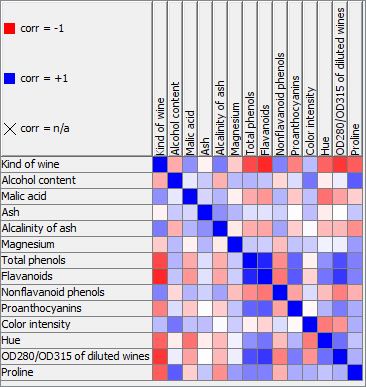
\includegraphics[width=0.75\textwidth]{wine-linear-correlation.png}
        \captionof{figure}{The linear correlation matrix of the wine data}\label{fig:wine-lin-corr}
      \end{answerfigure}

      Notable correlations include:
      \begin{itemize}
        \item the positive correlation between the wine's total phenols and the wine's flavanoids
        \item the negative correlation between the wine's type (technically a coincidence based on the possible arbitrary numbering) and the wine's total phenols and flavanoids
      \end{itemize}

      \newpage

      Based on the previous observations, let's visually confirm the correlations by observing the line plots of the mentioned attributes previously, as seen in Figure~\ref{fig:wine-line-plots}.

      \begin{answerfigure}
        \captionsetup{type=figure}
        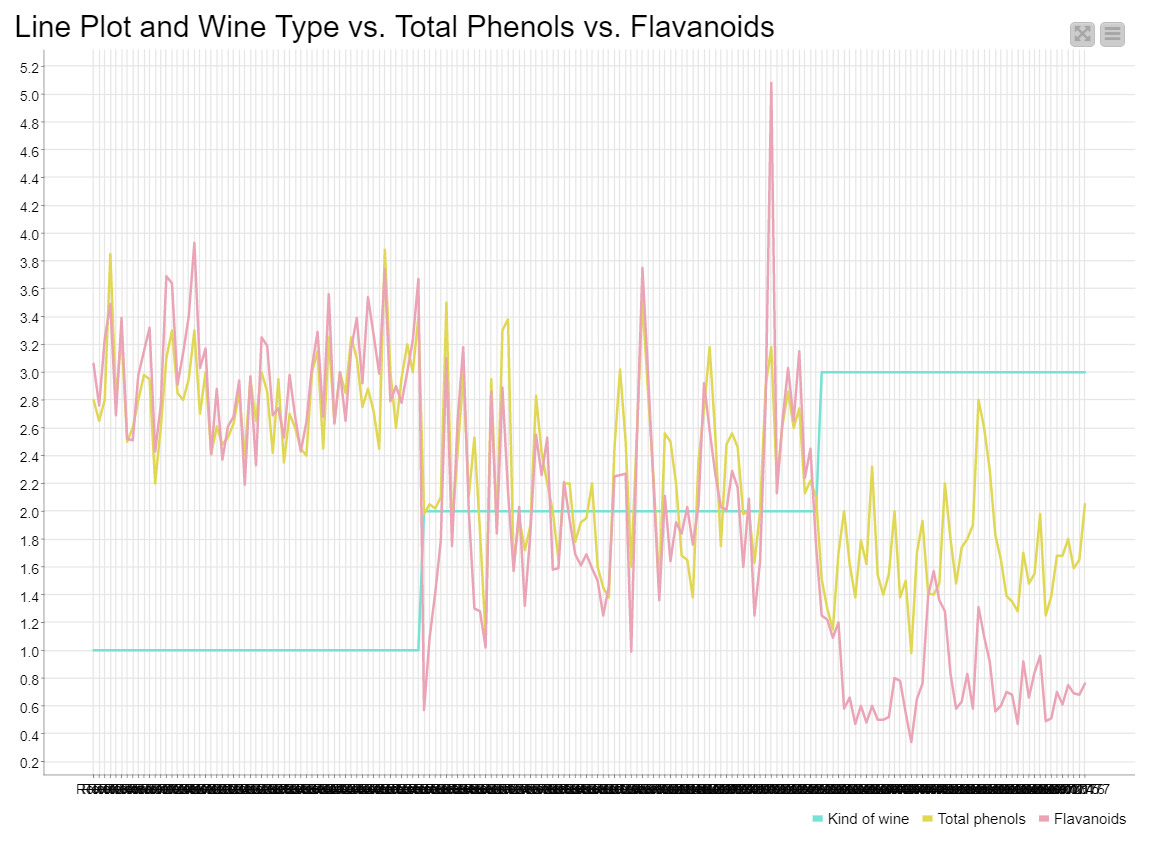
\includegraphics[width=\textwidth]{wine-line-plots.png}
        \captionof{figure}{The line plots of the Total phenols, Flavanoids, and the wine's type from the wine data}\label{fig:wine-line-plots}
      \end{answerfigure}

      It is clear that the correlation between the wine's total phenols and the wine's flavanoids is positive and that the correlation between the wine's type and the wine's total phenols/flavanoids is negative.

      Using the Statistics Node provided by KNIME, we can also generate a table of all the means, standard deviations, and min/max values for each attribute, as seen in Figure~\ref{fig:wine-stats}.

      \newpage
      \begin{center}
        \captionsetup{type=figure}
        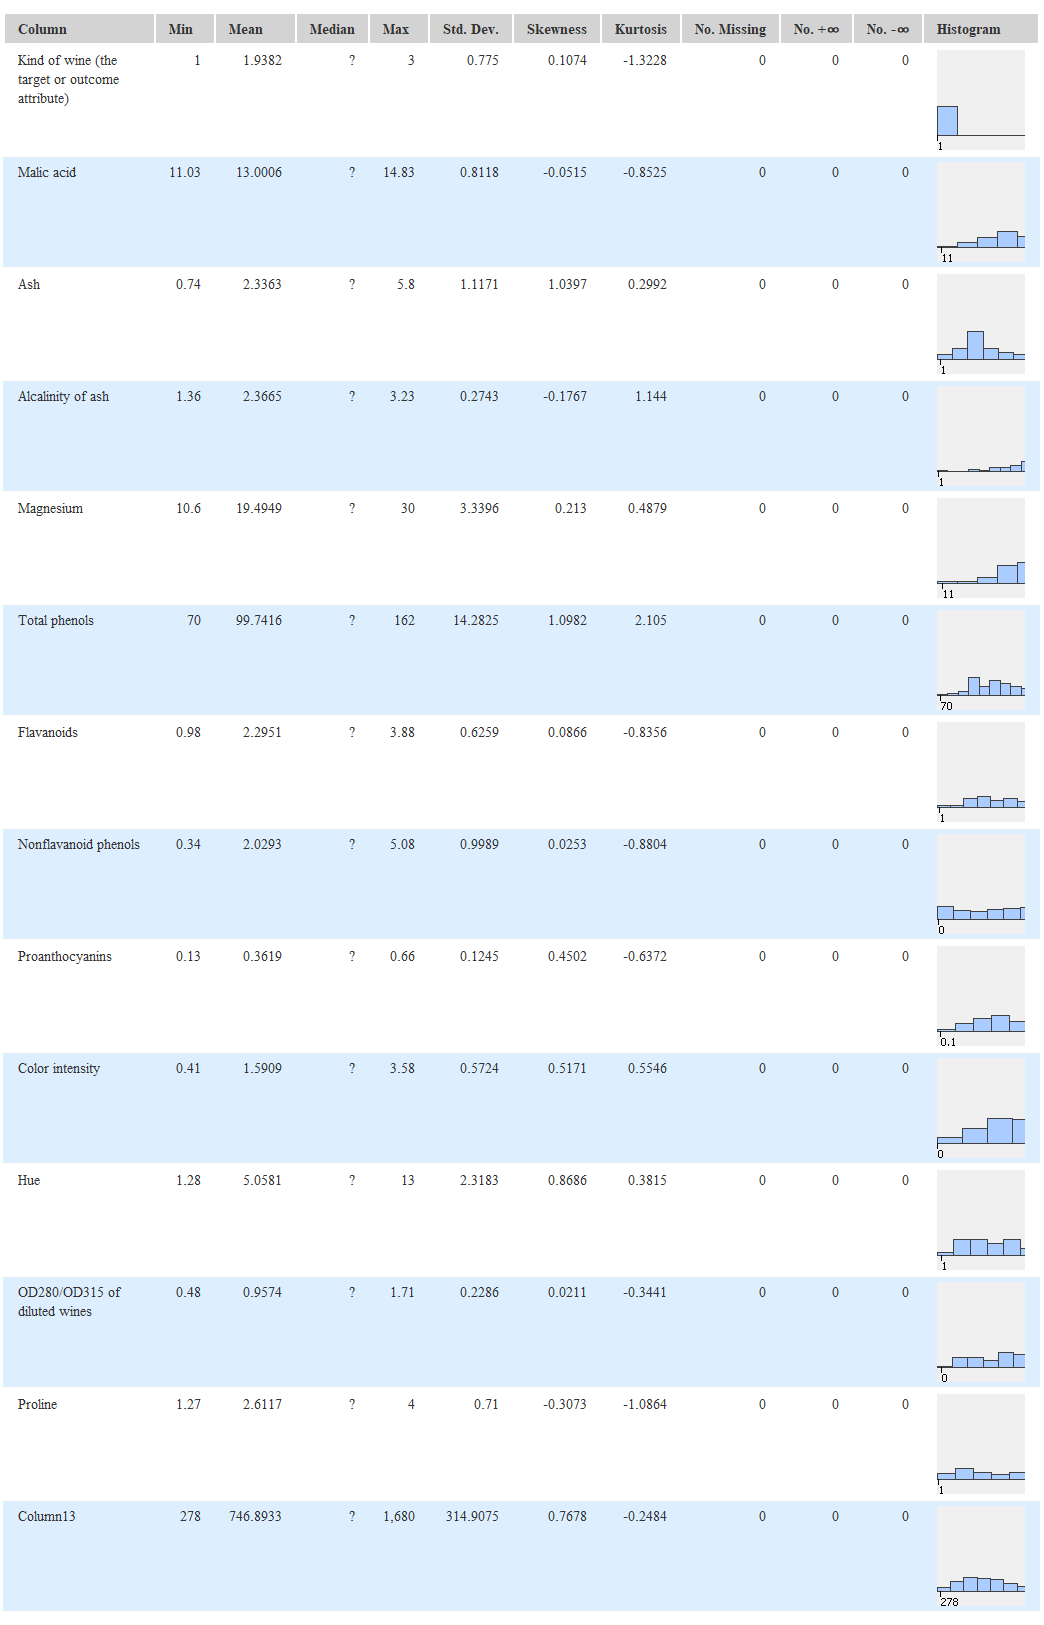
\includegraphics[width=0.8\textwidth]{wine-statistics.png}
        \captionof{figure}{General statistics of the wine data}\label{fig:wine-stats}
      \end{center}
    \end{solution}
  \end{questions}
\end{document}
